\section{Machine Learning}

The Machine Learning approach was to teach the neural network to recognize good tracks
 from a large list of candidates. 
 Two neural networks were developed: a classifier network that can identify good track from  6 segment
 track candidates  and an auto-encoder that can take a list of 5 segment tracks and make them into 6 segment 
 track candidates by adding a pseudo-segment. The composed 6 super-layer track candidates (with pseudo-cluster)
 can be processed with classifier network to identify and isolate "good" track candidates.

 %The implementation consisted of two neural networks: a classifier network
 %that can identify good track from  6 segment track candidates  and a auto-encoder that can take a list of
 %5 segment tracks and make them into 6 segment track candidates by adding a pseudo-segment.
 
 \subsection{Track Classifier}
 
 To determine what type of architecture works best with CLAS12 drift chamber data we investigated different 
 types of neural network including Convolutional Neural Network (CNN) , Extremely Randomized Trees (ERT) and 
 Multi-Layer Perceptron (MLP) \cite{Gavalian:2020oxg}. The study showed that Multi-Layer Perceptron was best suited for 
 CLAS12 reconstruction needs (based on inference speed and accuracy). The implemented architecture is shown on 
 Figure~\ref{mlp:architecture}, where an input layer with 6 nodes is used (each node representing average wire position 
 of the segment in super-layer) and 3 output nodes for classes "positive track", " negative track" and "false track".
 
 \begin{figure}[!ht]
\begin{center}
% 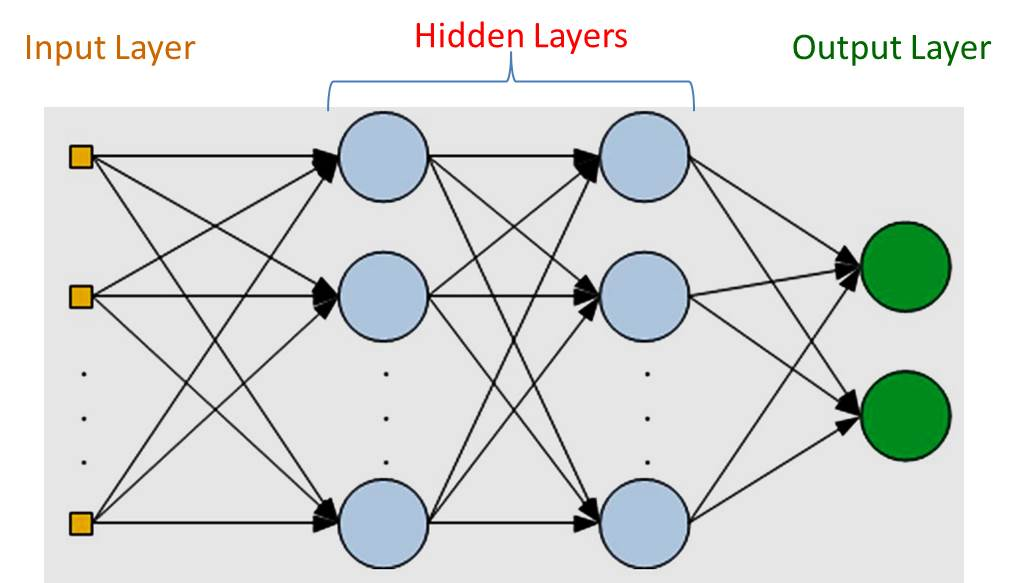
\includegraphics[width=3.5in]{images/Multilayer-Perceptron.jpg}
  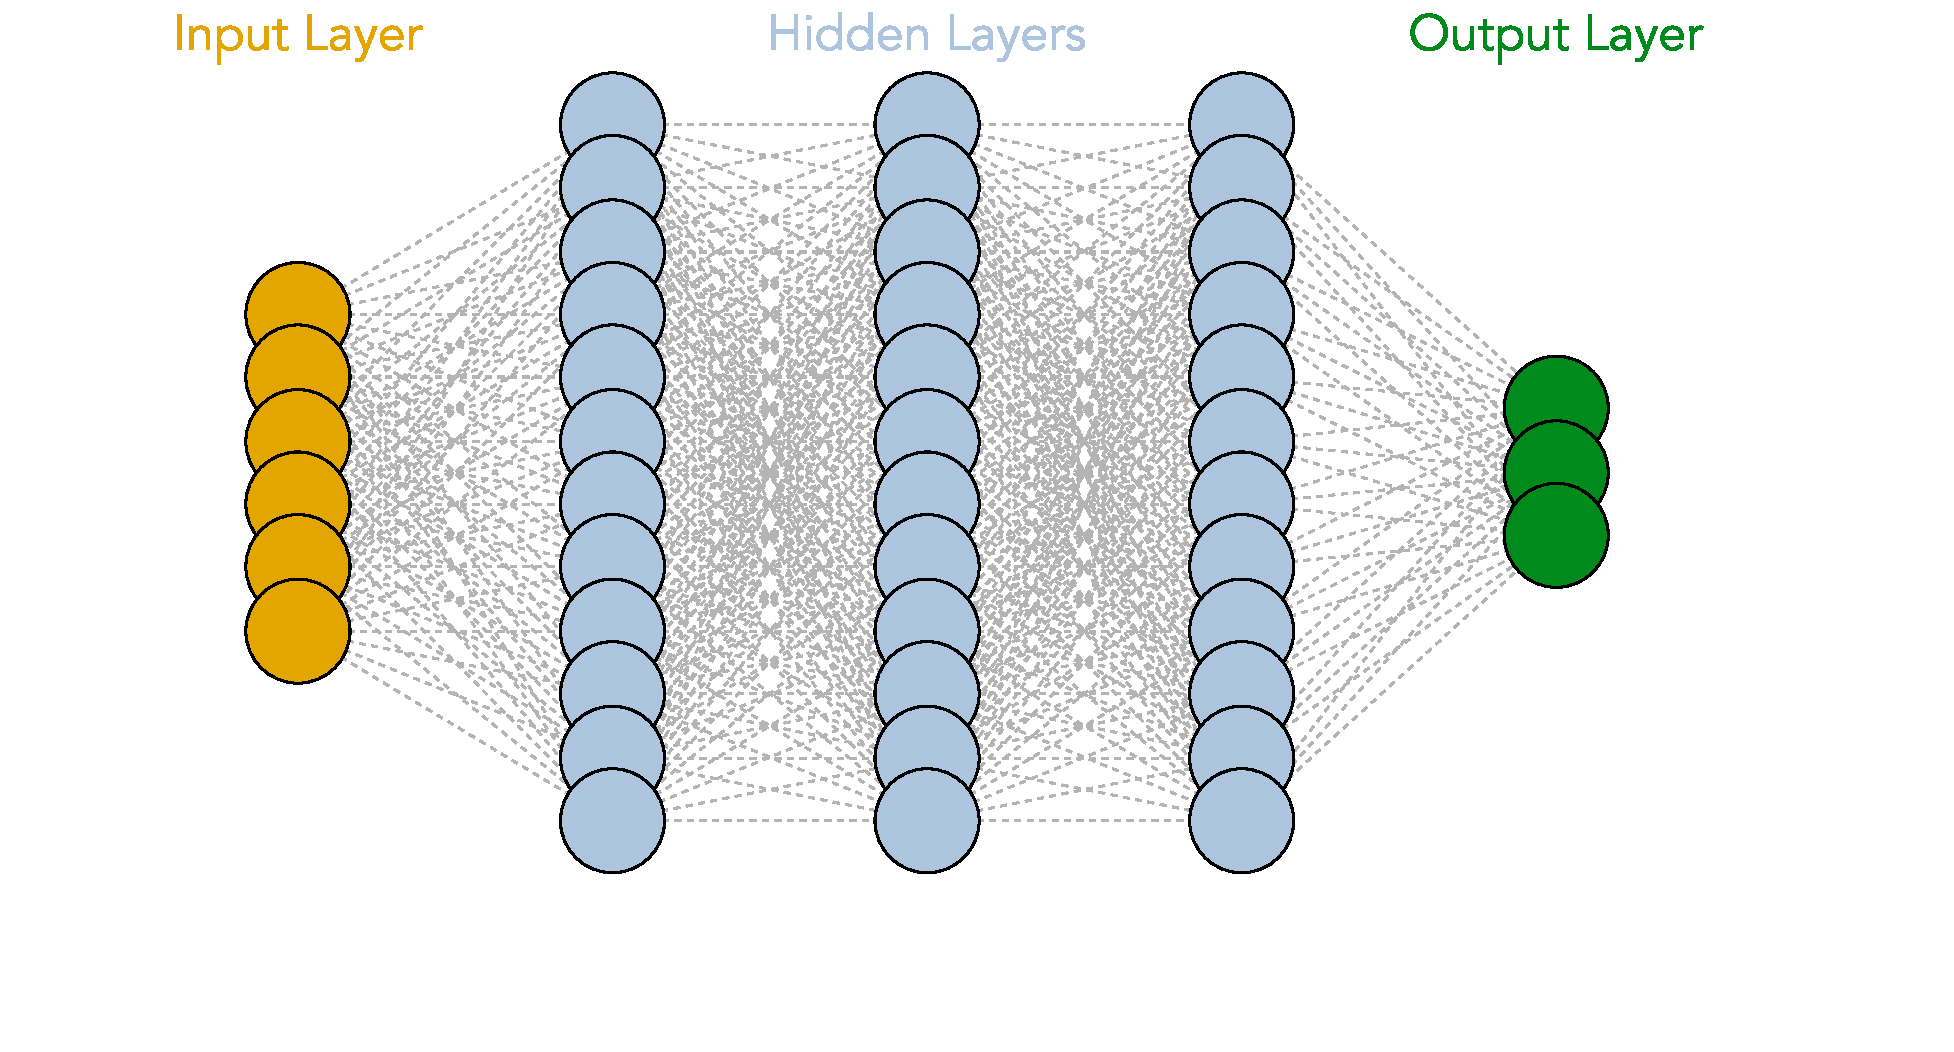
\includegraphics[width=5.0in]{images/mlp_diagram.pdf}
% 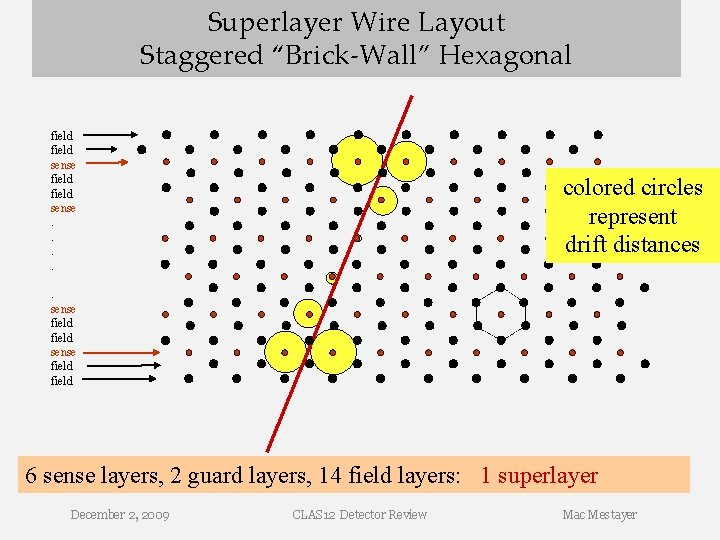
\includegraphics[width=2.5in]{images/image-29.jpg}
\caption {Architecture of Multi-Layer Perceptron used for track classification. Network has 6 input nodes, corresponding to average wire position of the segment in each super-layer, three hidden layers with 12 nodes in each and 3 output nodes.}
 \label{mlp:architecture}
 \end{center}
\end{figure}

The network is trained using results from processed data where the conventional algorithm has already 
identified good tracks (with a cut on $\chi^2$ to select very good quality tracks), which are fed to the network with
their respective labels (i.e. positive or negative tracks). For false tracks a combination of segments (6 segments 
forming a track candidate) is chosen that was not identified as a track by conventional algorithm.
 
 \subsection{Corruption Auto-Encoder}
 
The second neural network was developed to fix the corruption in possible track candidates due to 
inefficiencies of drift chambers. This network will be used to identify track candidates which have one of the segments
missing. We used auto-encoder type of neural network to implement feature fixing neural network \cite{Gavalian:2020xmc}. 
The structure of the network can be seen on Figure~\ref{autoencoder:architecture}, with 6 input nodes and six output nodes.

 \begin{figure}[!ht]
\begin{center}
 %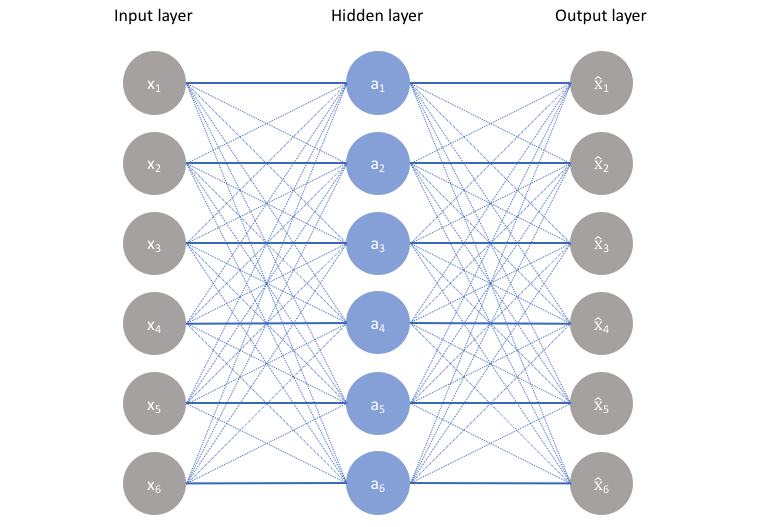
\includegraphics[width=2.0in]{images/auto_encoder.png}
%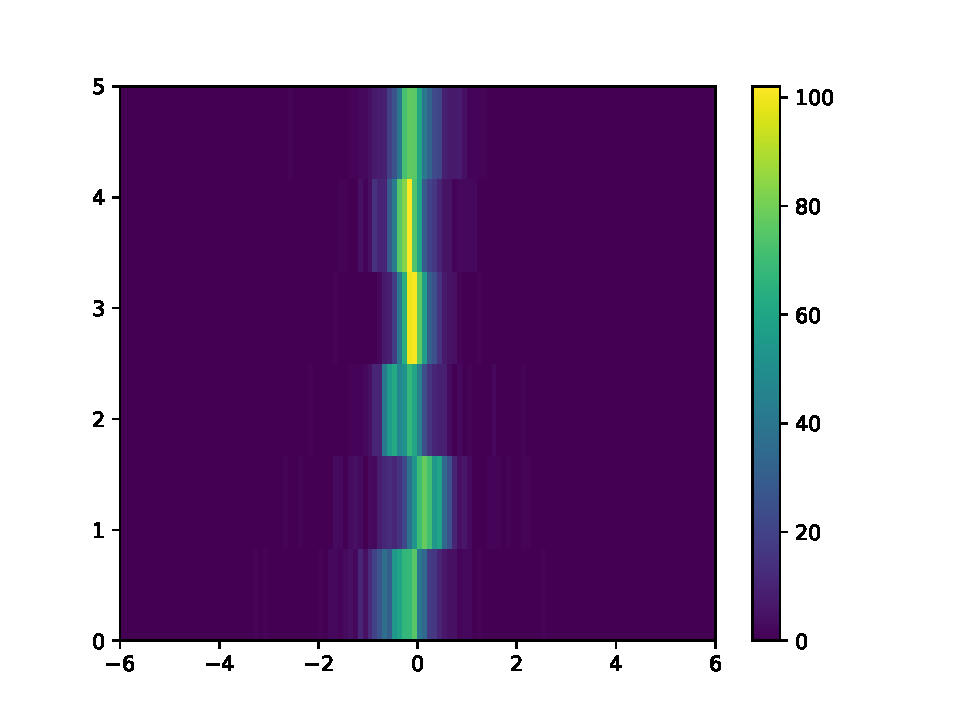
\includegraphics[width=2.0in]{images/auto_encoder_result_2d.pdf}
%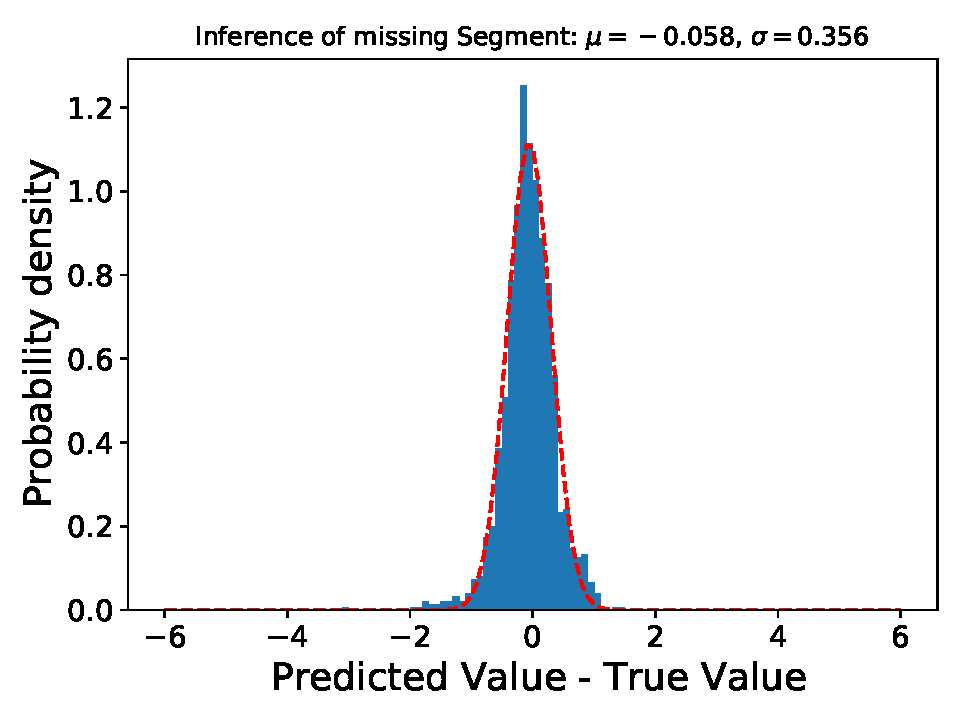
\includegraphics[width=2.0in]{images/auto_encoder_result_1d.pdf}
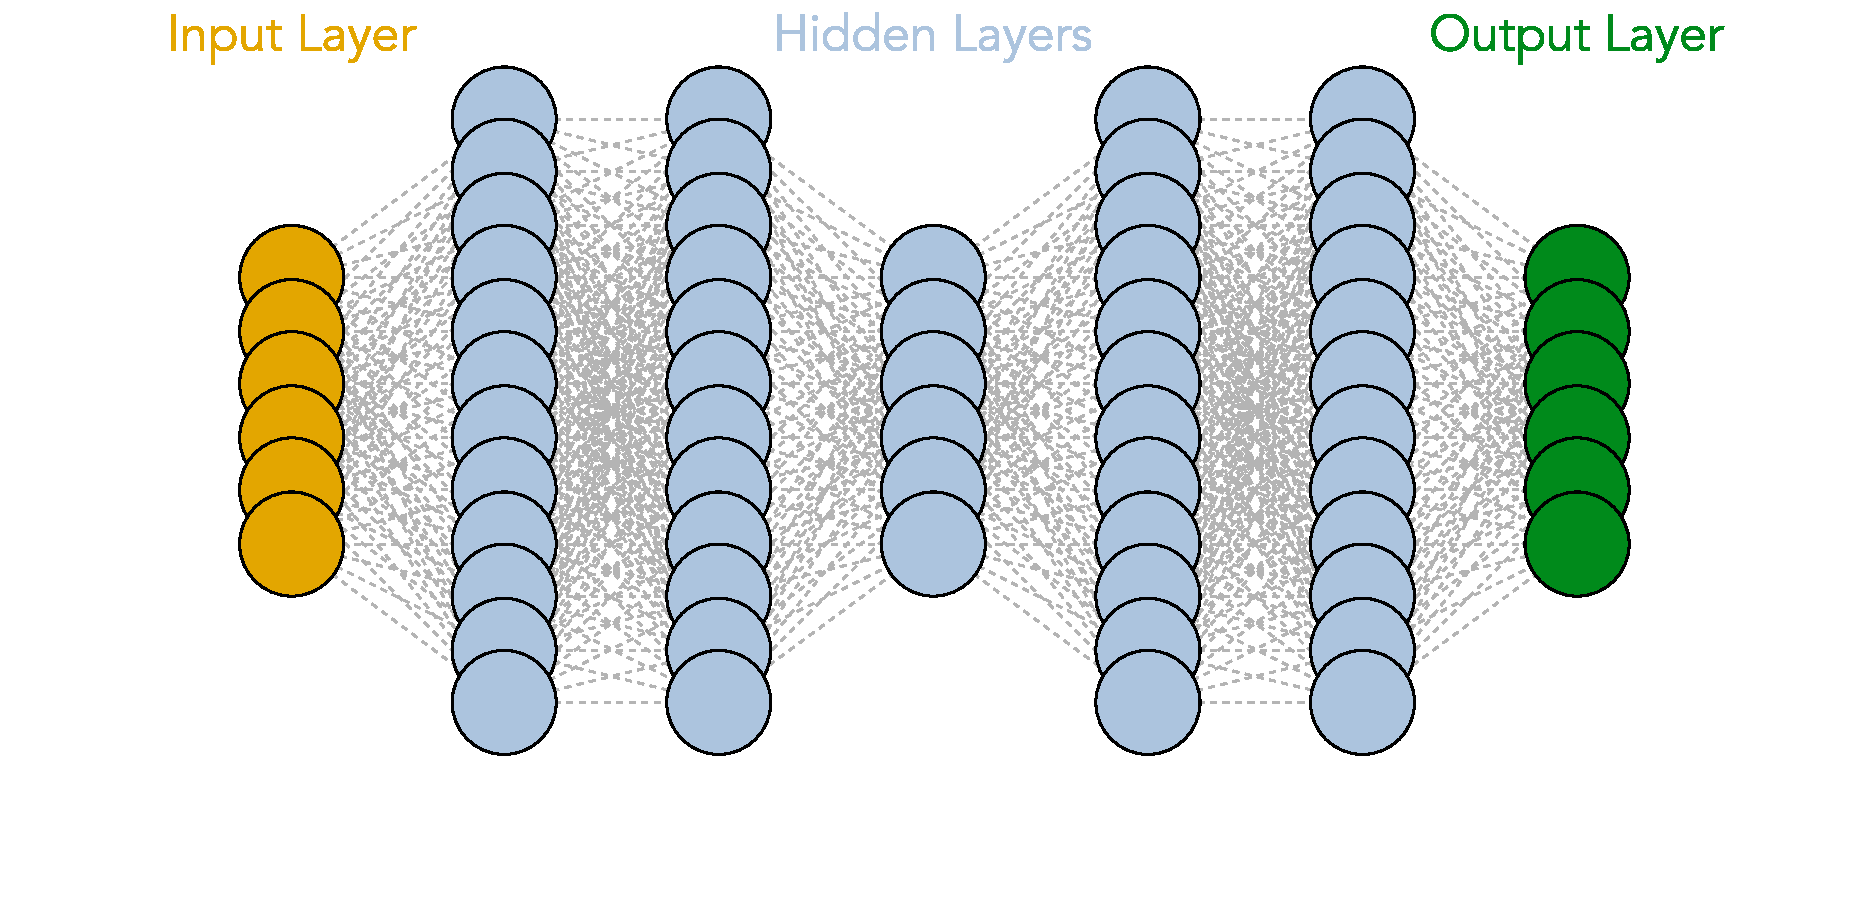
\includegraphics[width=5.0in]{images/aue_diagram.pdf}
\caption {Corruption recovery auto-encoder architecture with 6 input nodes representing track segments mean wire values with one of the values is set to 0, and 6 output nodes with the correct value for the node that has 0 in the input. }
 \label{autoencoder:architecture}
 \end{center}
\end{figure}

To train the network good track candidates reconstructed by conventional tracking algorithm are used (same sample 
as for track classifier network training). The output for the network was set to the good track parameters (where all 6 
segments have non-zero values) and the input was modified by setting one of the nodes (randomly) to zero. The network
learns to fix the node containing zero by assigning it a value based on the other 5 segment values. 
 \begin{figure}[!ht]
\begin{center}
 %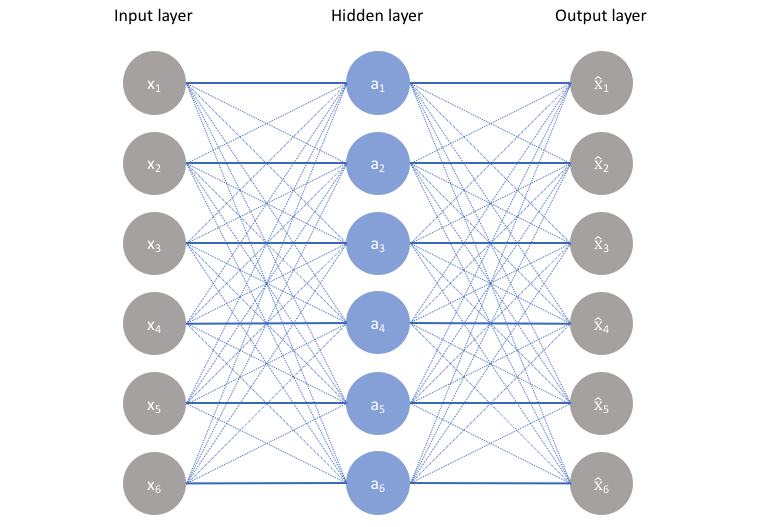
\includegraphics[width=2.0in]{images/auto_encoder.png}
%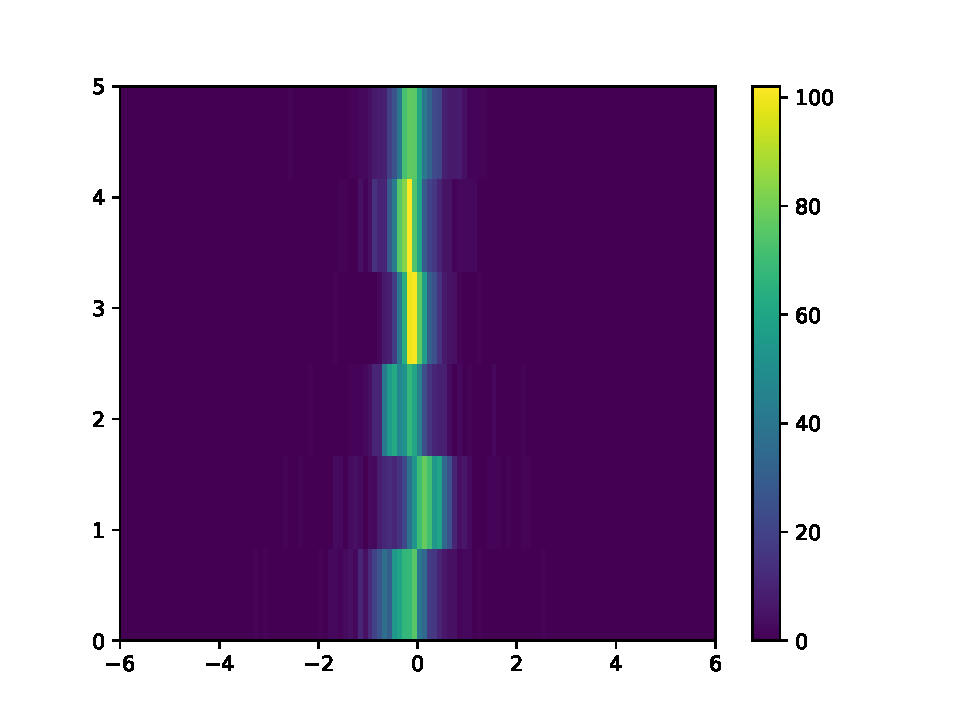
\includegraphics[width=2.0in]{images/auto_encoder_result_2d.pdf}
%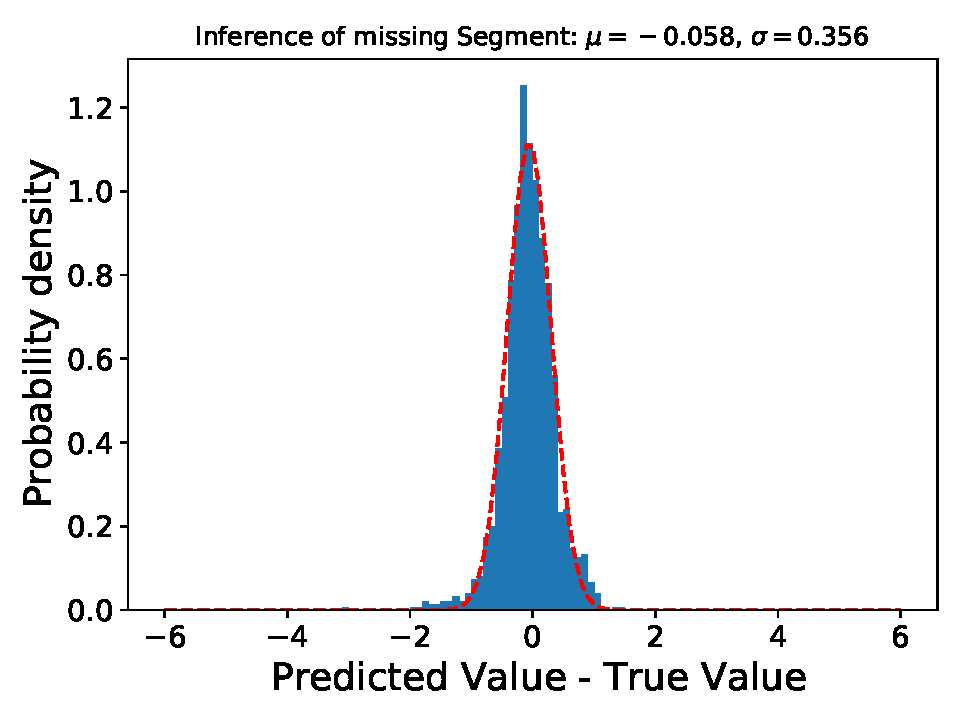
\includegraphics[width=2.0in]{images/auto_encoder_result_1d.pdf}
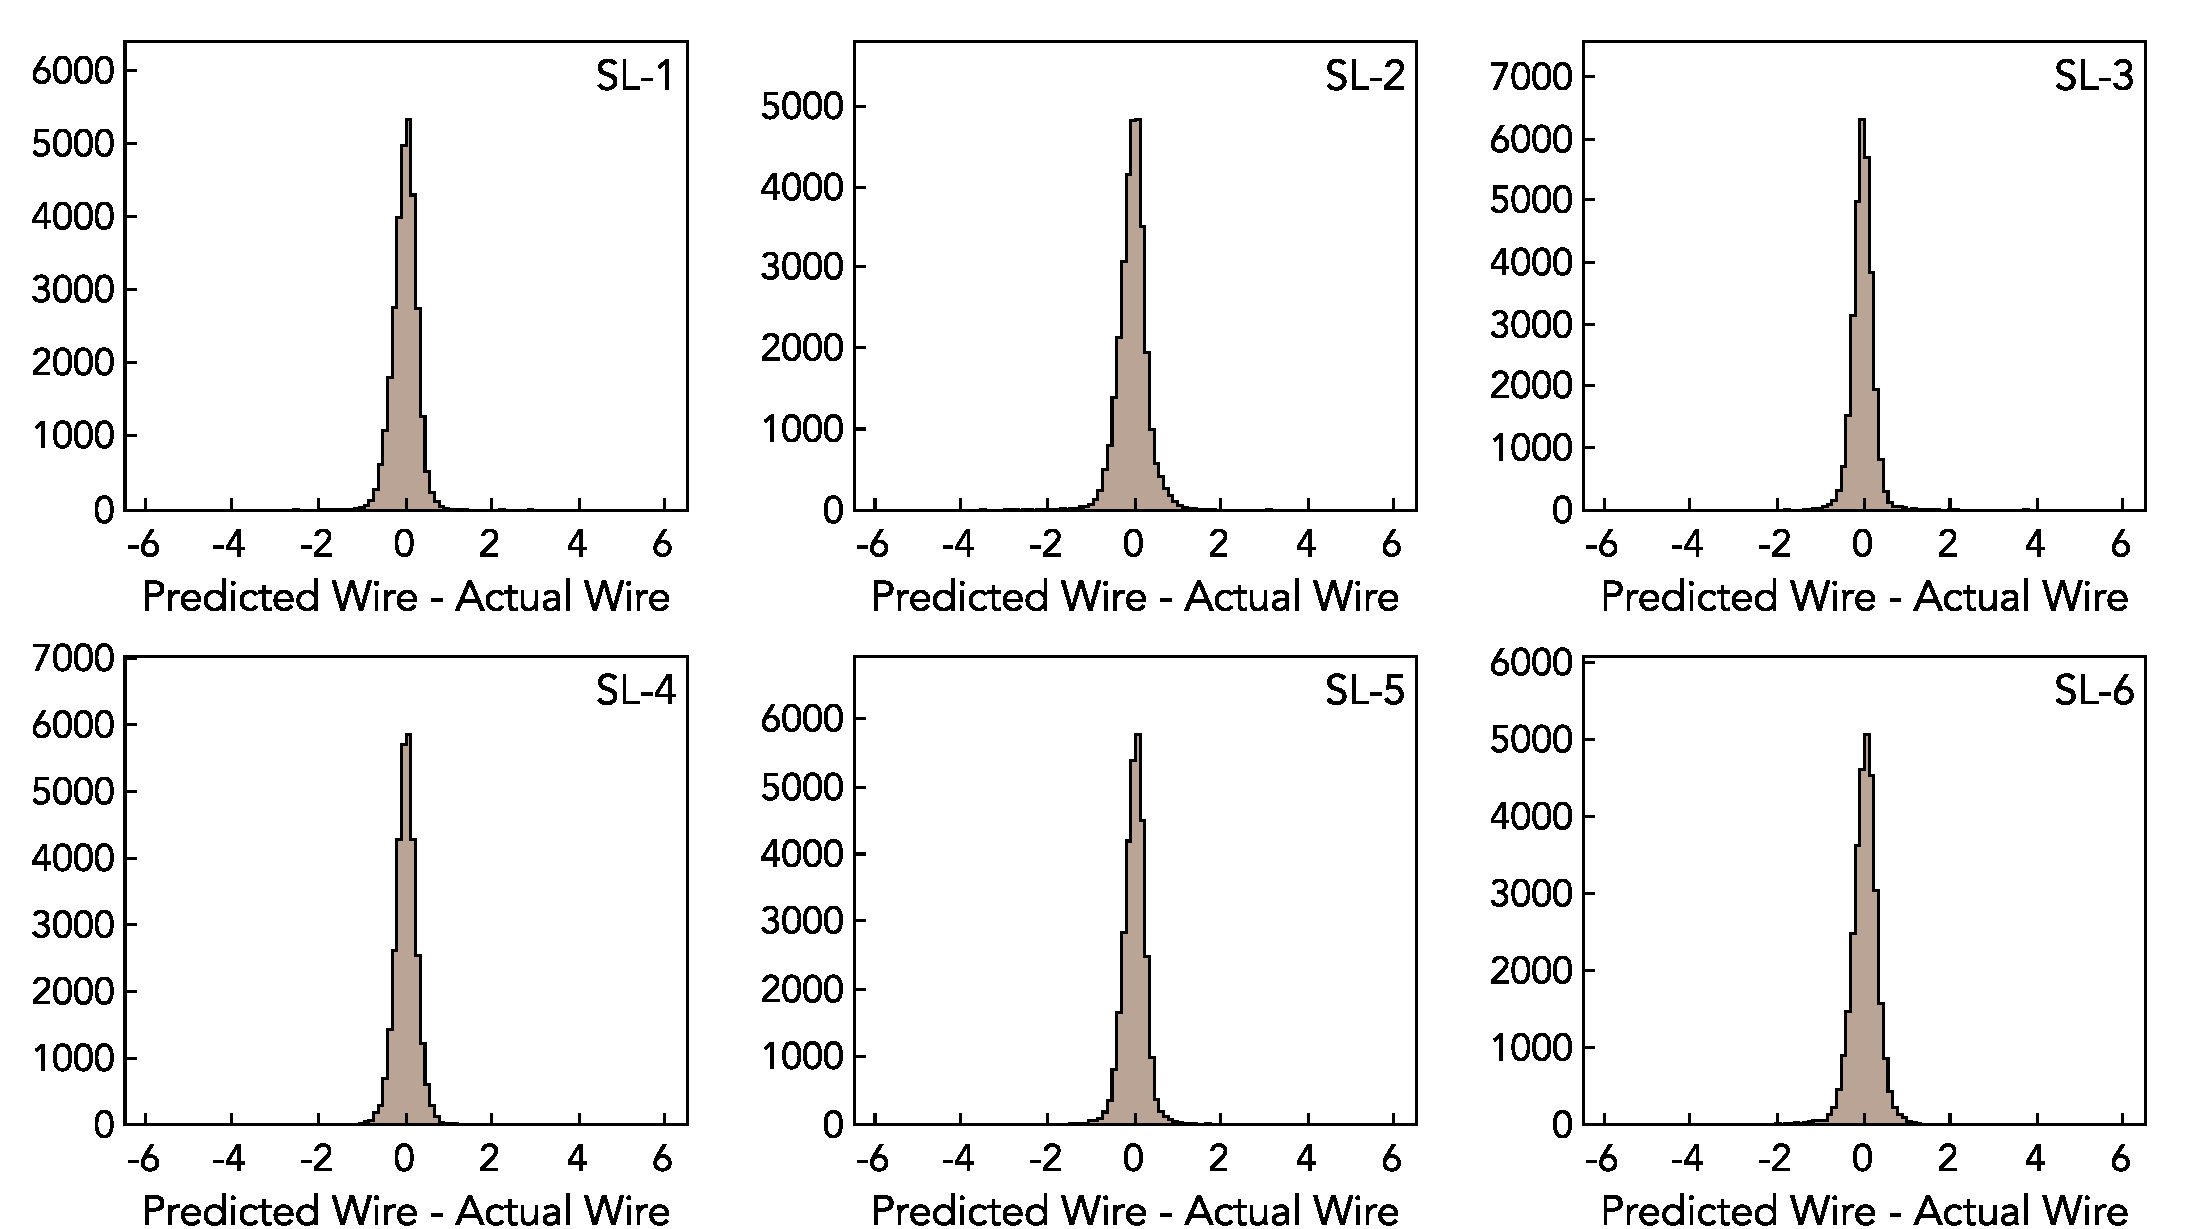
\includegraphics[width=6.0in]{images/encoder_performance.pdf}
\caption {Performance of corruption recovery auto-encoder. The difference between predicted and actual wire position 
is shown for all super-layers. Average accuracy of wire position prediction is  $0.36$ wire.}
 \label{autoencoder:performance}
 \end{center}
\end{figure}
The test results of the trained network are shown on Figure~\ref{autoencoder:architecture}, where the difference between true value 
of the segment position and reconstructed by network position is plotted, showing reconstruction accuracy of $0.36$ wires.
On Figure~\ref{autoencoder:architecture} this difference is shown vs the super-layer number which was corrupted in the input, 
as can be seen the performance of the network is uniform across all super-layers.



%\subsection{Implementation in reconstruction software}
%The CLAS12 track reconstruction software consist of several parts. The first stage of the process is to isolate clusters
%from the hits in drift chambers (called clustering service) . Once the clusters are isolated track candidates are formed from all combinations 
%of 6 segments. The track candidates are analyzed to determine which good candidates, from remaining segments 
%combinations of 5 segment tracks are constructed and these are also fitted to determine which ones are potential good tracks.
%The later module (hit based tracking) determines good track candidates based only on hit positions of the track candidates (no timing
%informations is used at this level). At the later stages of tracking code (time based tracking), chosen good track candidates are further refined by use of Kalman filter by using timing information from each of the sensors (drift chamber wires). By the time the reconstruction code reaches time based
%tracking stage the track candidates are already defined. 

%\begin{figure}[!ht]
%\begin{center}
% 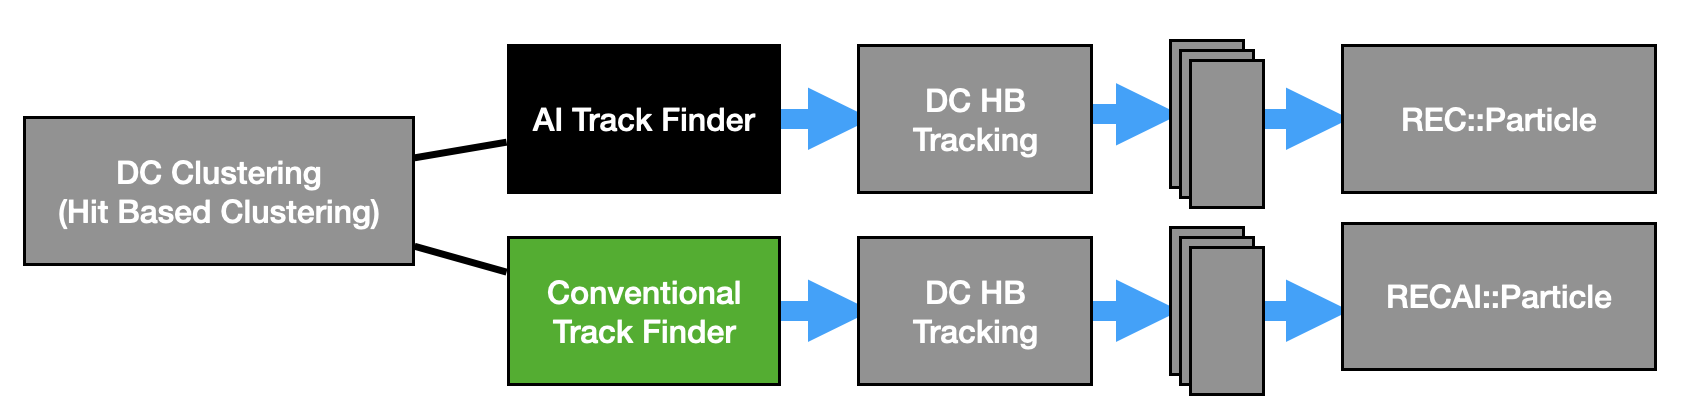
\includegraphics[width=6.0in]{images/recon_diagram.png}
%\caption {Architecture of corruption fixing Auto-Encoder.}
% \label{recon:diagram}
% \end{center}
%\end{figure}

%In order to implement our neural network into reconstruction workflow we designed two parallel branches in reconstruction code where we run 
%two algorithms to identify good tracks from track candidate lists, one based on conventional algorithm and second based on neural network.
%Both algorithms store their track suggestions in separate data structures, and pass them to the next stage where track parameters are reconstructed by 
%conventional tracking algorithm using Kalman filter. This approach let's us have two parallel outputs from tracking code in order to compare performance of
%each of the methods.
